\documentclass[report]{subfiles}
\begin{document}










% Dora Start

\section{Winner-take-all circuit (WTA)}
\subsection{How does the WTA circuit work?}

The circuit of Fig. \ref{fig:WTA} is a continuous time, analog circuit that implements
a WTA network, designed by Lazzaro et al. (1989).

It processes all the (continuous-time) input signals in
parallel, using only two transistors per input cell, and one global transistor
that is common to all cells. Collective computation and global connectivity is
obtained using one single node common to all cells.

\begin{figure}[htbp]
  \centering
  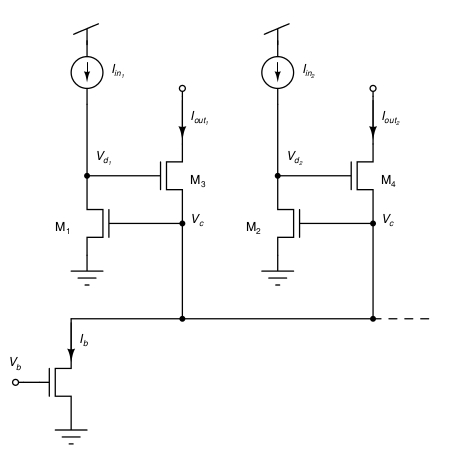
\includegraphics[scale=0.8]{pics/WTA.jpg}
  \caption{Two cells of a current mode WTA circuit \cite{book:VLSI}.}
  \label{fig:WTA}
\end{figure} 

The WTA network is modular and can be extended to n cells. 

Each cell comprises a current-controlled conveyor as in figure \ref{fig:current_conveyor}. The inputs of the circuit are applied currents,
output signals are encoded both by $I_{out}$ currents, and the $V_d$ voltages. 

\begin{figure}[htbp]
  \centering
  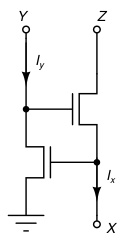
\includegraphics[scale=0.8]{pics/current_conveyor.jpg}
  \caption{Current-controlled conveyor \cite{book:VLSI}.}
  \label{fig:current_conveyor}
\end{figure} 

The application -- current coping in which the current-conveyor circuit is used in WTA is showed in the figure \ref{fig:current_conveyor_application}. Before to copy a current we used the current-mirror. It is very efficient -- as we need 1 transistor less. However, as the output of the circuit is connected in feed-back loop to the input, the sum of parasitic capacitances $C_{gs}$ will significantly slow down the output. In the most drastic case the outputs will even not detect any change in input current signal -- for high frequency time variant inputs (slew-rates limites output respond, higher time constant $\tau = RC$).

\begin{figure}[htbp]
  \centering
  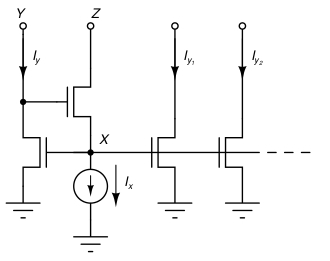
\includegraphics[scale=0.8]{pics/current_conveyor_application.jpg}
  \caption{System application of current conveyor for the generation of multiple copies of an input current \cite{book:VLSI}.}
  \label{fig:current_conveyor_application}
\end{figure} 

Transistors $M_1$ and $M_2$ discharge nodes $V_d$ -- implement inhibitory feedback. Transistors $M_3$ and $M_4$
 implement an excitatory feed-forward path by charging node $V_c$ . 
 
 The circuit selects the largest input current because cell provides j provides $I_{out}^j = I_b$  and so suppresses all other output voltages and currents (all other $V_d \approx 0$ and $I_{out} \approx 0$). Cell j wins the competition because its voltage $V_d^j$
determines $V_c$ ($V_{gs}$ is set by fixed value of $I_b$). Since all cells have common $V_c$ gate potentials it will be grater than $V_d$ for all other cells than j -- they will be shut-off \cite{book:VLSI}. 




\textit{Briefly: the circuit chooses one winner by selecting a cell with the highest input current (max() function). All other cells are suppressed (inhibited).}

Hysteretic WTA: by feeding back the output of the circuit to its input, the system gets more stable and less sensitive to probable new winner.

\subsection{Can you reason through its behaviour?}
We consider three cases (the network with two cells): 

\begin{enumerate}[label={I.}]
\item inputs are equal; 
\item one input much larger than the other; 
\item two inputs differ by a very small amount (small-signal regime).
\end{enumerate}

\begin{enumerate}[label={I.}]
\item Because gates of $M_1$ and $M_2$ are tied to the same common node $V_c$, the drain voltages of $M_1$ and $M_2$ must take the same value. As a result, the output transistors $M_3$ and $M_4$ will have equal $V_{gs}$ value and in case both of them are in saturation, the output currents have to be identical. Upon Kirchhoff's current law:
\begin{equation}
I_{out_1} = I_{out_2} = \frac{I_b}{2} 
\end{equation}

\item 

We can consider the case in which $I_{in_1}\gg I_{in_2}$. In this case, the drain voltage of $M_1$ ($V_{d_1}$) will be greater than the drain voltage of $M_2$ ($V_{d_2}$).

Because the two transistors $M_1$ and $M_2$ have a common gate voltage $V_c$, and both their sources are tied to ground, the froward current (dependent only on $V_{gs}$) for both them is equal. The need to suppress the value of forward current through $M_2$ arises. Therefore voltage $V_{d_2}$ has to be decreased (lower current for the same gate-to-source voltage ). We say that reverse current -- dependent only on $V_{ds}$ -- will increase, limiting overall current through drain to $I_{in_2}$ value. 

Decrease of $V_{d_2}$ causing $M_2$ to operate in its ohmic region (out of saturation), switches off $M_4$. This implies $I_{out_2}=0$. 

Consequently, output transistor $M_3$ sources all the bias current 
\begin{equation}
I_{out_1} = I_b,
\end{equation}
with $V_{d_1}$ satisfying the equation 
\begin{equation}
I_0 e^{\kappa V_{d_1}- V_c} = I_b.
\end{equation}

\item 
To analyze the circuit in this regime, we will use small-signal analysis. We must consider the Early effect of the transistor operating in the saturation region (Eq. \ref{eq:WTA_early_effect}):

\begin{equation}
I_{ds} = I_{sat}(1+ \frac{V_{ds}}{V_e})
\label{eq:WTA_early_effect}
\end{equation}
, $V_e$ is the Early voltage.
By derivating this equation (small-signal analysis) we get: $\delta I_{ds} = I_{sat} \frac{\delta V_{ds}}{V_e})$.

Assume that the two input currents $I_{in_1}$ and $I_{in_2}$ are initially equal. 

If we now increase the input current $I_{in_1}$ by a small amount $\delta I$ we would like to be able to obtain a difference in $M_1$ transistor's $V_{d_1}$, which is:
\begin{equation}
\delta V_d = \delta I_d \frac{V_e}{I_{sat}}
\end{equation}

As $V_{d_1}$ is also the gate voltage of transistor $M_3$, the $I_{out_1}$ will be amplified by an amount proportional to $e^{\delta V}$ . The Kirchhoff's law requires that
$I_{out_2}$ decreases by the same amount. This reduction means the gate voltage $V_{d_2}$ of $M_2$ must decrease by $\delta V$ \cite{book:VLSI}.
\end{enumerate}

All three cases can be summarised by the graphic \ref{fig:WTA_response}.

\begin{figure}[htbp]
  \centering
  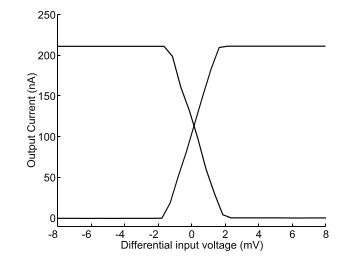
\includegraphics[scale=0.9]{pics/WTA_response.jpg}
  \caption{Responses of the two-cell WTA circuit. Current output ($I_{out_1}$ and $I_{out_2}$). The bias voltage $V_b = 0.7V$ \cite{book:VLSI}.}
  \label{fig:WTA_response}
\end{figure} 

\subsection{How does the bias current affect its performance?}
With increasing bias current it will get harder to choose a winner -- it takes larger input current difference to suppress all cells excluding the winner. 

???
\subsection{How can you adjust the gain of the circuit by layout of the transistors?}
Since the gain in the small-signal regime of the competition of the WTA circuit is expressed by equation:
\begin{equation}
\frac{\delta V}{\delta I} = \frac{V_e}{I_{sat}} 
\end{equation}
the only transistors' layout variables are early Voltage $V_e$ (dependent on the length of transistor) and $I_0$ coefficient of the saturation current (linearly dependent on $W/L$). Therefore, we can increase the gain by decreasing the width of the transistor or by increasing its length. 

???
\end{document}